\begin{abox}
	Practice Set- 1
\end{abox}
\begin{enumerate}
	\item A time varying signal $V_{i n}$ is fed to an op-amp circuit with output signal $V_{o}$ as shown in the figure below.\\
	\begin{figure}[H]
		\centering
		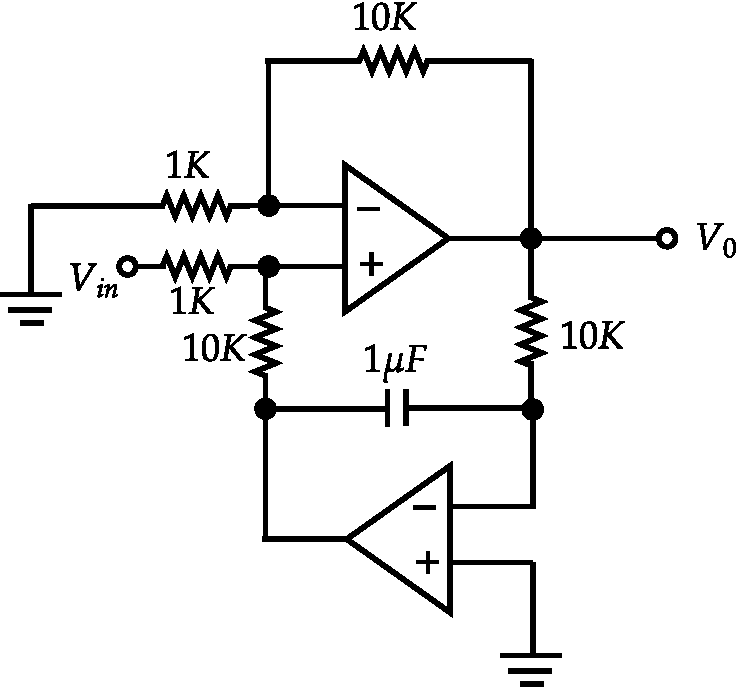
\includegraphics[height=6cm,width=6.5cm]{diagram-20211018(1)-crop}
	\end{figure}
	The circuit implements a
	{\exyear{NET/JRF(JUNE-2011)}}
	\begin{tasks}(1)
		\task[\textbf{A.}] High pass filter with cutoff frequency $16 \mathrm{~Hz}$
		\task[\textbf{B.}] High pass filter with cutoff frequency $100 \mathrm{~Hz}$
		\task[\textbf{C.}] Low pass filter with cutoff frequency $16 \mathrm{~Hz}$
		\task[\textbf{D.}] Low pass filter with cutoff frequency $100 \mathrm{~Hz}$
	\end{tasks}
\begin{answer}
	\begin{align*}
	\intertext{Since circuit has $R$ and $C$ combination, its a Low Pass filter and cutoff frequency}
	&=\frac{1}{2 \pi R C} \approx 16 H z
	\end{align*}
	So the correct answer is \textbf{Option (C)}
\end{answer}
	\item In the operational amplifier circuit below, the voltage at point $A$ is
	{	\exyear{NET/JRF(DEC-2011)}}
	\begin{figure}[H]
		\centering
		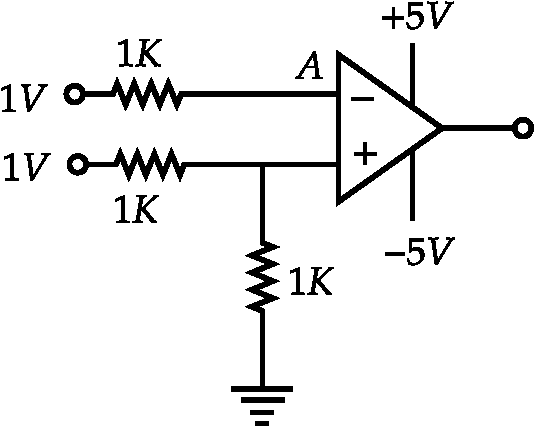
\includegraphics[height=4cm,width=5.5cm]{diagram-20211018(2)-crop}
	\end{figure}
	\begin{tasks}(4)
		\task[\textbf{A.}] $1.0 \mathrm{~V}$
		\task[\textbf{B.}] $0.5 \mathrm{~V}$
		\task[\textbf{C.}] $0 \mathrm{~V}$
		\task[\textbf{D.}] $-5.0 V$
	\end{tasks}
\begin{answer}
	\begin{align*}
	V_{A}&=\frac{1}{1+1} \times 1=0.5 \mathrm{~V}
	\end{align*}
	So the correct answer is \textbf{Option (B)}
\end{answer}
	\item In the op-amp circuit shown in the figure below, the input voltage is $1 \mathrm{~V}$. The value of the output $\mathrm{V}_{0}$ is
	{\exyear{NET/JRF(JUNE-2012)}}
	\begin{figure}[H]
		\centering
		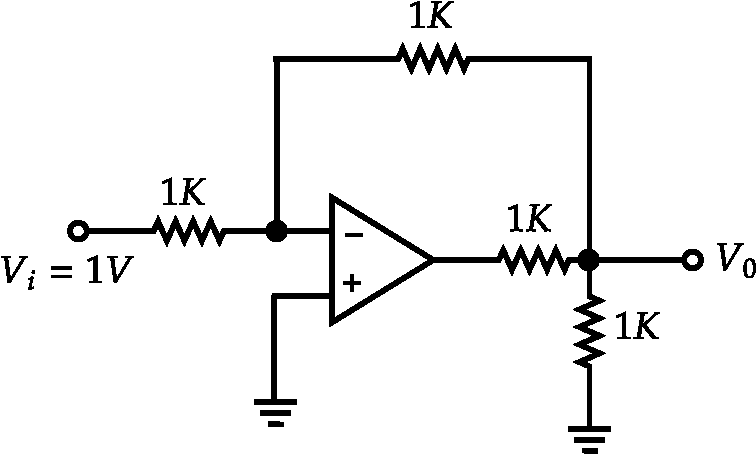
\includegraphics[height=3.5cm,width=6cm]{e-08}
	\end{figure}
	\begin{tasks}(4)
		\task[\textbf{A.}] $-0.33 \mathrm{~V}$
		\task[\textbf{B.}] $-0.50 \mathrm{~V}$
		\task[\textbf{C.}] $-1.00 \mathrm{~V}$
		\task[\textbf{D.}] $-0.25 \mathrm{~V}$
	\end{tasks}
\begin{answer}
	\begin{align*}
	V_{0}&=-\frac{R_{F} V_{i n}}{R_{1}}=-\frac{1}{2} V=-0.05\\\text{ where }R_{F}&=\frac{1 \times 1}{1+1}=\frac{1}{2} K and R_{1}=1 K
	\end{align*}
	So the correct answer is \textbf{Option (B)}
\end{answer}
	\item In the op-amp circuit shown in the figure, $V_{i}$ is a sinusoidal input signal of frequency 10 $\mathrm{Hz}$ and $V_{0}$ is the output signal. The magnitude of the gain and the phase shift, respectively, close to the values
	{	\exyear{NET/JRF(DEC-2012)}}
		\begin{tasks}(1)
			\task[\textbf{A.}] $5 \sqrt{2}$ and $\pi / 2$
			\task[\textbf{B.}] $5 \sqrt{2}$ and $-\pi / 2$
			\task[\textbf{C.}] 10 and zero
			\task[\textbf{D.}] 10 and $\pi$
		\end{tasks}
	\begin{answer}
		\begin{align*}
		\frac{v_{0}}{v_{i n}}
		&=-\frac{X_{C} R_{F}}{R_{1}\left(R_{1}+R_{F}\right)} \Rightarrow\left|\frac{v_{0}}{v_{i n}}\right| \approx 10
		\end{align*}
		So the correct answer is \textbf{Option (D)}
	\end{answer}
		\begin{figure}[H]
			\centering
			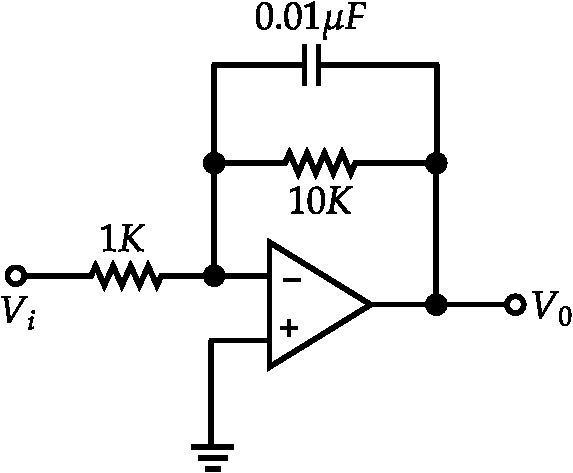
\includegraphics[height=4cm,width=5cm]{e-13}
		\end{figure}
	\item Consider the op-amp circuit shown in the figure.
	If the input is a sinusoidal wave $V_{i}=5 \sin (1000 t)$, then the amplitude of the output $V_{0}$ is
	{	\exyear{NET/JRF(DEC-2013)}}
	\begin{figure}[H]
		\centering
		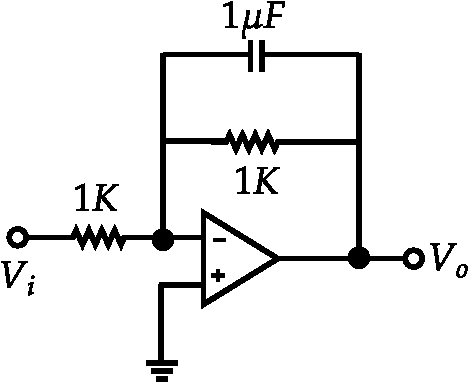
\includegraphics[height=3.5cm,width=4.5cm]{e-21}
	\end{figure}
	\begin{tasks}(4)
		\task[\textbf{A.}] $\frac{5}{2}$
		\task[\textbf{B.}]  5
		\task[\textbf{C.}] $\frac{5 \sqrt{2}}{2}$
		\task[\textbf{D.}] $5 \sqrt{2}$
	\end{tasks}
\begin{answer}
	\begin{align*}
	\frac{v_{o}}{v_{\text {in }}}&=-\frac{X_{F}}{R_{1}}, X_{F}=\frac{R_{F} X_{C}}{R_{F}+X_{C}}=\frac{10^{3}}{(1+j)}\\\text{ where }R_{F}&=1 \times 10^{3} \Omega, X_{C}=\frac{1}{j \times 10^{3} \times 10^{-6}}\\
	\left|\frac{v_{o}}{v_{i n}}\right|&=\frac{10^{3}}{\sqrt{2}} \times \frac{1}{10^{3}}=\frac{1}{\sqrt{2}} \Rightarrow v_{o}\\&=\frac{5}{\sqrt{2}} \sin \omega t=\frac{5 \sqrt{2}}{2} \sin \omega t
	\end{align*}
	So the correct answer is \textbf{Option (C)}
\end{answer}
	\item The inner shield of a triaxial conductor is driven by an (ideal) op-amp follower circuit as shown. The effective capacitance between the signal-carrying conductor and ground is
	{	\exyear{NET/JRF(JUNE-2014)}}
	\begin{figure}[H]
		\centering
		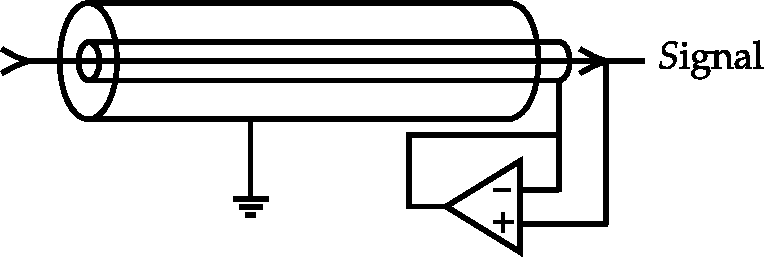
\includegraphics[height=2.5cm,width=7cm]{e-26}
	\end{figure}
	\begin{tasks}(4)
		\task[\textbf{A.}]  Unaffected
		\task[\textbf{B.}] Doubled
		\task[\textbf{C.}] Halved
		\task[\textbf{D.}] Made zero
	\end{tasks}
\begin{answer}
	So the correct answer is \textbf{Option (A)}
\end{answer}
	\item Consider the amplifier circuit comprising of the two op-amps $A_{1}$ and $A_{2}$ as shown in the in the figure. \\
	\begin{figure}[H]
		\centering
		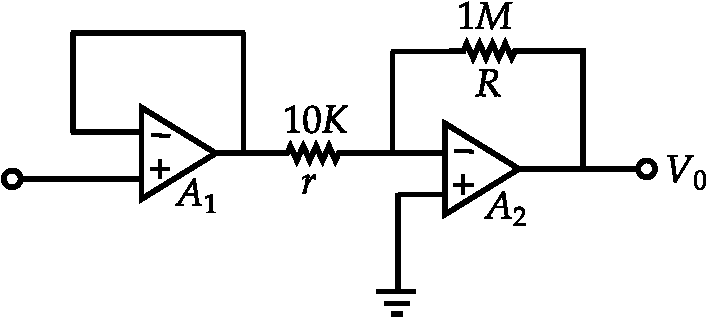
\includegraphics[height=3cm,width=7cm]{e-30}
	\end{figure}
	If the input ac signal source has an impedance of $50 k \Omega$, which of the following statements is true?
	{	\exyear{NET/JRF(DEC-2014)}}
	\begin{tasks}(1)
		\task[\textbf{A.}] $A_{1}$ is required in the circuit because the source impedance is much greater than $r$
		\task[\textbf{B.}] $A_{1}$ is required in the circuit because the source impedance is much less than $R$
		\task[\textbf{C.}] $A_{1}$ can be eliminated from the circuit without affecting the overall gain
		\task[\textbf{D.}] $A_{1}$ is required in the circuit if the output has to follow the phase of the input signal
	\end{tasks}
\begin{answer}$\left. \right. $\\
	$A_{1}$ is required in the circuit because the source impedance is much greater than $r$\\
	So the correct answer is \textbf{Option (A)}
\end{answer}
	\item Consider a Low Pass (LP) and a High Pass (HP) filter with cut-off frequencies $f_{L P}$ and $f_{H P}$, respectively, connected in series or in parallel configurations as shown in the Figures A and B below.\\
	\begin{figure}[H]
		\centering
		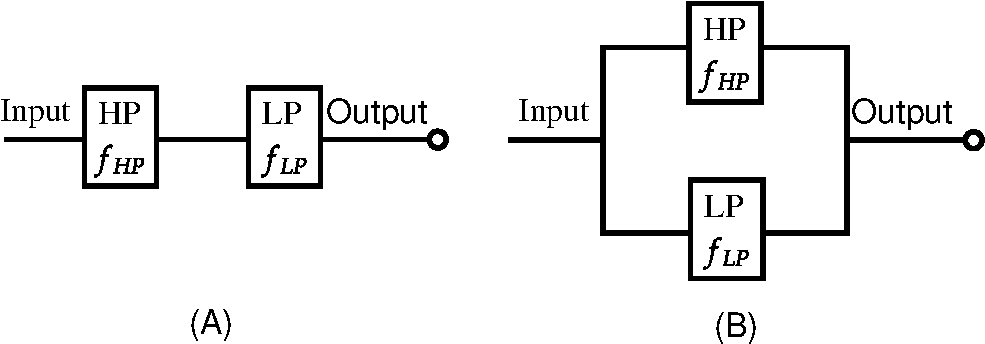
\includegraphics[height=3cm,width=10cm]{e-33}
	\end{figure}
	Which of the following statements is correct?
	{	\exyear{NET/JRF(DEC-2014)}}
	\begin{tasks}(1)
		\task[\textbf{A.}] For $f_{H P}<f_{L P}$, A acts as a Band Pass filter and B acts as a band Reject filter
		\task[\textbf{B.}] For $f_{H P}>f_{L P}$, A stops the signal from passing through and B passes the signal without filtering
		\task[\textbf{C.}] For $f_{H P}<f_{L P}$, A acts as a Band Pass filter and B passes the signal without filtering
		\task[\textbf{D.}] For $f_{H P}>f_{L P}$, A passes the signal without filtering and B acts as a Band Reject filter
	\end{tasks}
\begin{answer}
	So the correct answer is \textbf{Option (C)}
\end{answer}
	\item In the circuit given below, the thermistor has a resistance $3 k \Omega$ at $25^{0} C$. Its resistance decreases by $150 \Omega$ per ${ }^{0} C$ upon heating. The output voltage of the circuit at $30^{\circ} \mathrm{C}$ is
	{	\exyear{NET/JRF(JUNE-2015)}}
	\begin{figure}[H]
		\centering
		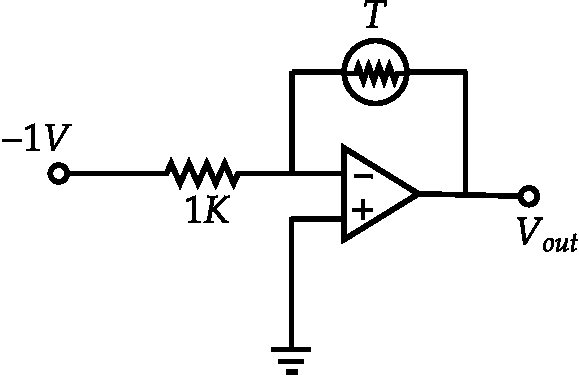
\includegraphics[height=3.3cm,width=5.5cm]{e-38}
	\end{figure}
	\begin{tasks}(4)
		\task[\textbf{A.}] $-3.75 \mathrm{~V}$
		\task[\textbf{B.}] $-2.25 \mathrm{~V}$
		\task[\textbf{C.}] $2.25 \mathrm{~V}$
		\task[\textbf{D.}] $3.75 \mathrm{~V}$
	\end{tasks}
\begin{answer}
	\begin{align*}
	\text{At }30^{\circ} C,\text{ Resistance }&=3000-150 \times 5=2250 \Omega\\
	\Rightarrow V_{0}&=-\frac{R_{F}}{R_{1}} v_{i}=\frac{-2250}{1000} \times-1 \Rightarrow V_{0}=2.25\text{ volts}
	\end{align*}
	So the correct answer is \textbf{Option (C)}
\end{answer}
	\item If the parameters $y$ and $x$ are related by $y=\log (x)$, then the circuit that can be used to produce an output voltage $V_{0}$ varying linearly with $x$ is
	{\exyear{NET/JRF(DEC-2015)}}
	\begin{tasks}(2)
		\task[\textbf{A.}] \begin{figure}[H]
			\centering
			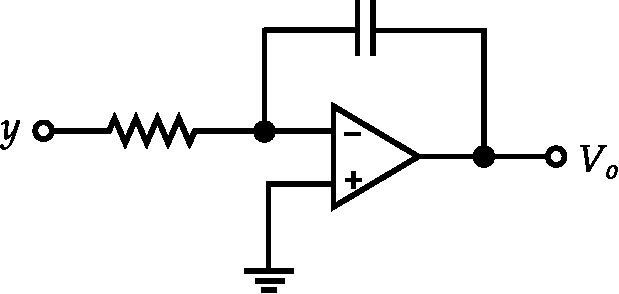
\includegraphics[height=3cm,width=5.5cm]{e40a}
		\end{figure}
		\task[\textbf{B.}] \begin{figure}[H]
			\centering
			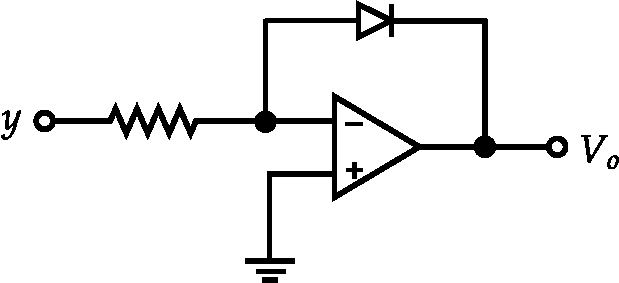
\includegraphics[height=3cm,width=5.5cm]{e40b}
		\end{figure}
		\task[\textbf{C.}] \begin{figure}[H]
			\centering
			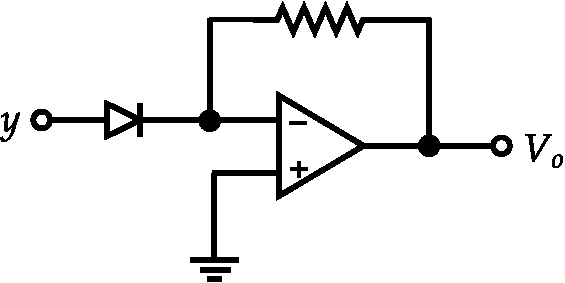
\includegraphics[height=3cm,width=5.5cm]{e40c}
		\end{figure}
		\task[\textbf{D.}] \begin{figure}[H]
			\centering
			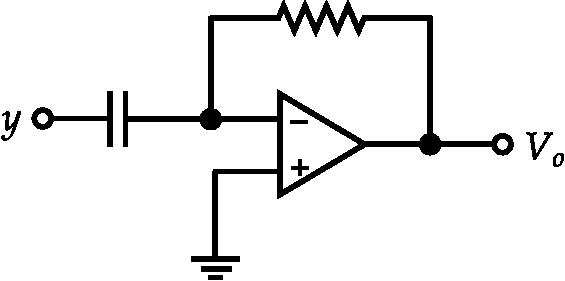
\includegraphics[height=3cm,width=5.5cm]{e40d}
		\end{figure}
	\end{tasks}
\begin{answer}$\left. \right. $\\
	(1) Integrator\\
	(2) Logarithmic Ampere $\left(V_{0} \propto \log y\right)$\\
	(3) Anti-log $\left(V_{0} \propto e^{y} \propto x\right)$\\
	(4) Differentiator\\
	So the correct answer is \textbf{Option (C)}
\end{answer}
	\item A sinusoidal signal of peak to peak amplitude $1 V$ and unknown time period is input to the following circuit for 5 second's duration. If the counter measures a value $(3 E 8)_{H}$ in hexadecimal, then the time period of the input signal is
	{	\exyear{NET/JRF(DEC-2015)}}
	\begin{figure}[H]
		\centering
		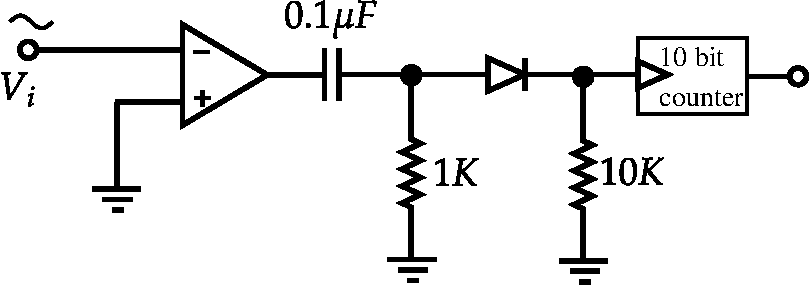
\includegraphics[height=3cm,width=8cm]{e42}
	\end{figure}
	\begin{tasks}(4)
		\task[\textbf{A.}] $2.5 \mathrm{~ms}$
		\task[\textbf{B.}] $4 \mathrm{~ms}$
		\task[\textbf{C.}]  $10 \mathrm{~ms}$
		\task[\textbf{D.}] $5 \mathrm{~ms}$
	\end{tasks}
\begin{answer}
	\begin{align*}
	(3 E 8)_{H} \rightarrow 3 \times 16^{2}+14 \times 16+8 \times 1&=(1000)_{10}
	\intertext{In $5 \mathrm{sec}$, number of counts is 1000 .}
	\text{Then count per sec is }&=200\text{ count/sec}\\
	\text{So, }T&=\frac{1}{200} \sec =5 m s
	\end{align*}
	So the correct answer is \textbf{Option (D)}
\end{answer}
	\item Given the input voltage $V_{i}$, which of the following waveforms correctly represents the output voltage $V_{0}$ in the circuit shown below?
	{	\exyear{NET/JRF(JUNE-2016)}}
	\begin{figure}[H]
		\centering
		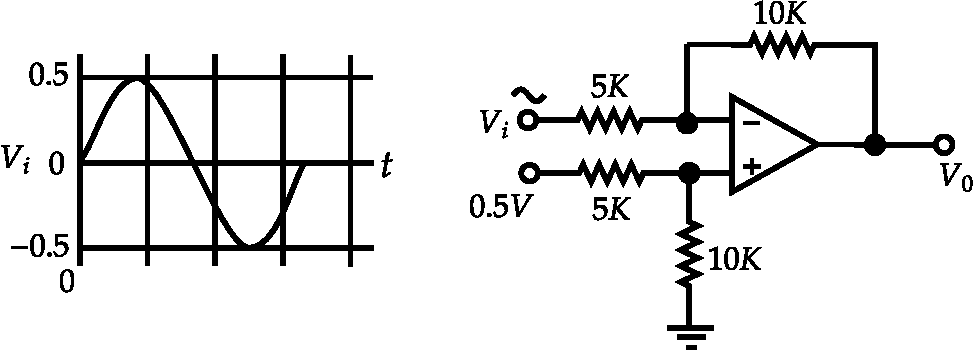
\includegraphics[height=3.5cm,width=10cm]{diagram-20211020(13)-crop}
	\end{figure}
	\begin{tasks}(2)
		\task[\textbf{A.}] \begin{figure}[H]
			\centering
			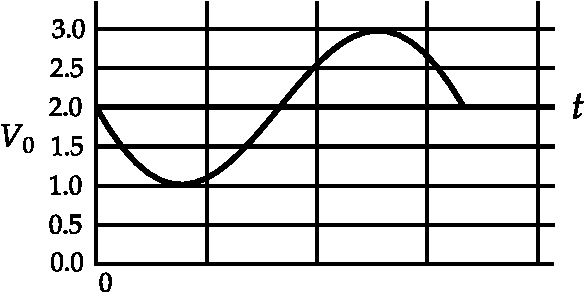
\includegraphics[height=3cm,width=5.5cm]{diagram-20211020(14)-crop}
		\end{figure}
		\task[\textbf{B.}] \begin{figure}[H]
			\centering
			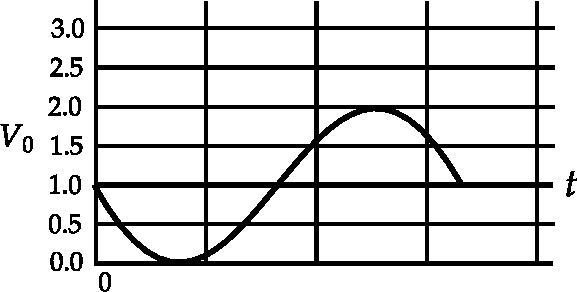
\includegraphics[height=3cm,width=5.5cm]{diagram-20211020(15)-crop}
		\end{figure}
		\task[\textbf{C.}] \begin{figure}[H]
			\centering
			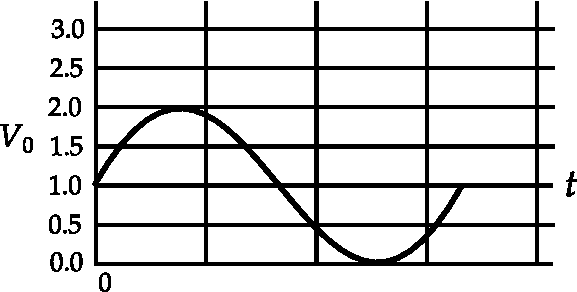
\includegraphics[height=3cm,width=5.5cm]{diagram-20211020(16)-crop}
		\end{figure}
		\task[\textbf{D.}] \begin{figure}[H]
			\centering
			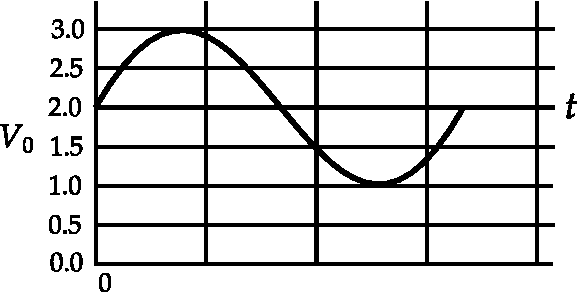
\includegraphics[height=3cm,width=5.5cm]{diagram-20211020(17)-crop}
		\end{figure}
	\end{tasks}
\begin{answer}
	\begin{align*}
	V_{0}&=\left(1+\frac{10}{5}\right) \times \frac{10}{15} \times 0.5-\frac{10}{5} \times V_{i} \Rightarrow V_{0}=1-2 V_{i}
	\intertext{When $V_{i}=0 \Rightarrow V_{0}=1 V$, when $V_{i}=0.1 V \Rightarrow V_{0}=0.8 V$, when $V_{i}=0.5 V \Rightarrow V_{0}=0 V$}
	\end{align*}
	So the correct answer is \textbf{Option (B)}
\end{answer}
	\item  In the circuit below, the input voltage $V_{i}$ is $2 V, V_{c c}=16 \mathrm{~V}, R_{2}=2 \mathrm{k} \Omega$ and $R_{L}=10 \mathrm{k} \Omega$\\
	\begin{figure}[H]
		\centering
		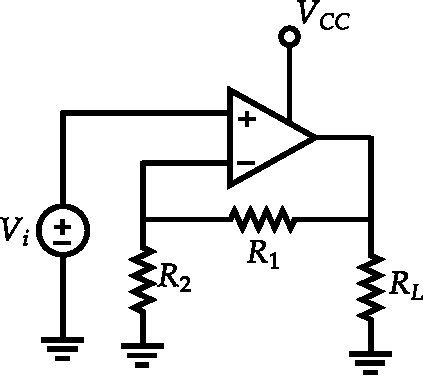
\includegraphics[height=3.5cm,width=4.5cm]{e50}
	\end{figure}
	The value of $R_{1}$ required to deliver $10 \mathrm{~mW}$ of power across $R_{L}$ is
	{\exyear{NET/JRF(DEC-2016)}}
	\begin{tasks}(4)
		\task[\textbf{A.}] $12 k \Omega$
		\task[\textbf{B.}] $4 k \Omega$
		\task[\textbf{C.}]  $8 \mathrm{k} \Omega$
		\task[\textbf{D.}]  $14 k \Omega$
	\end{tasks}  
\begin{answer}$\left. \right. $
	\begin{figure}[H]
		\centering
		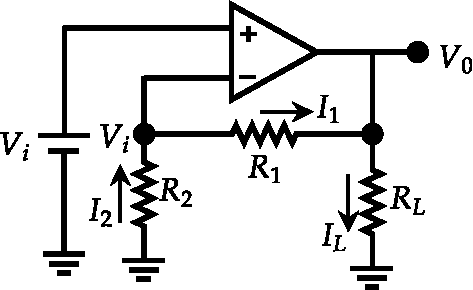
\includegraphics[height=3.2cm,width=5.5cm]{e50s}
	\end{figure}
	\begin{align*}
	\text{Apply }k C L ; I_{2}&=I_{1}=I_{L} \Rightarrow \frac{0-v_{i}}{R_{2}}=\frac{v_{i}-v_{0}}{R_{1}}=\frac{v_{0}-0}{R_{L}}\\
	p_{L}&=\frac{v_{0}^{2}}{R_{L}}=10 m W \Rightarrow v_{0}=10 V\\
	\Rightarrow \frac{0-2}{2}&=\frac{2-10}{R_{1}}=\frac{10 V}{10 k} \Rightarrow-1\\&=\frac{-8}{R_{1}} \Rightarrow R_{1}=8 k \Omega
	\end{align*}
	So the correct answer is \textbf{Option (C)}
\end{answer}              
	\item The gain of the circuit given below is $-\frac{1}{\omega R C}$.\\
	\begin{figure}[H]
		\centering
		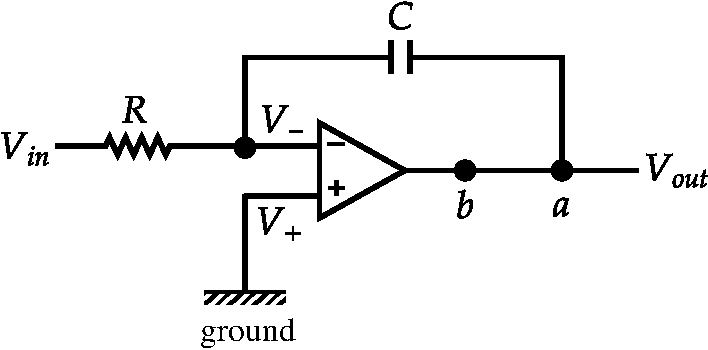
\includegraphics[height=3.5cm,width=6.5cm]{e54}
	\end{figure}
	The modification in the circuit required to introduce a dc feedback is to add a resistor
	{\exyear{NET/JRF(JUNE-2017)}}
	\begin{tasks}(1)
		\task[\textbf{A.}] Between $a$ and $b$
		\task[\textbf{B.}]  Between positive terminal of the op-amp and ground
		\task[\textbf{C.}] In series with $C$
		\task[\textbf{D.}] Parallel to $C$
	\end{tasks}
\begin{answer}
	So the correct answer is \textbf{Option (D)}
\end{answer}
	\item In the following operational amplifier circuit $C_{i n}=10 n F, R_{i n}=20 k \Omega, R_{F}=200 k \Omega$ and $C_{F}=100 \mathrm{pF}$\\
	\begin{figure}[H]
		\centering
		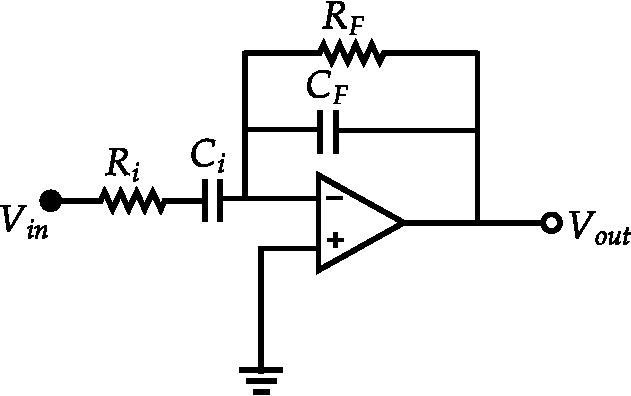
\includegraphics[height=3.5cm,width=6cm]{e60}
	\end{figure}
	The magnitude of the gain at a input signal frequency of $16 \mathrm{kHz}$ is
	{\exyear{NET/JRF(JUNE-2017)}}
	\begin{tasks}(4)
		\task[\textbf{A.}] 67
		\task[\textbf{B.}] $0.15$
		\task[\textbf{C.}] $0.3$
		\task[\textbf{D.}] $3.5$
	\end{tasks}
\begin{answer}
	\begin{align*}
	\frac{V_{o}}{V_{i n}}&=-\frac{z_{F}}{z_{i}}=-\frac{R_{F} \| X_{C_{F}}}{R_{i}+X_{C_{i}}}=-\frac{R_{F} \times \frac{1}{J \omega c_{F}} /\left(R_{F}+\frac{1}{J \omega c_{F}}\right)}{\left(R_{i}+\frac{1}{J \omega c_{i}}\right)}\\
	\frac{V_{o}}{V_{i n}}&=\frac{-R_{F} /\left(J \omega c_{F} R_{F}+1\right)}{\left(j \omega c_{i} R_{i}+1\right) / j \omega c_{i}}=\frac{-R_{F}}{\left(j \omega c_{F} R_{F}+1\right)} \times \frac{j \omega c_{i}}{\left(1+j \omega R_{i} c_{i}\right)}\\
	\Rightarrow\left|\frac{V_{o}}{V_{\text {in }}}\right|&=\frac{\omega c_{i} R_{F}}{\sqrt{1+\left(\omega c_{F} R_{F}\right)^{2}} \sqrt{1+\left(\omega R_{i} c_{i}\right)^{2}}}, \omega=2 \pi f
	\intertext{$\Rightarrow\left|\frac{V_{0}}{V_{\text {ln }}}\right|=\frac{\left(2 \pi \times 16 \times 10^{3}\right)\left(10 \times 10^{-9}\right)\left(200 \times 10^{3}\right)}{\sqrt{1+4 \pi^{2}\left(16 \times 10^{3}\right)^{2}\left(200 \times 10^{3}\right)^{2}\left(100 \times 10^{-12}\right)^{2}} \sqrt{1+4 \pi^{2}\left(16 \times 10^{3}\right)^{2}\left(20 \times 10^{3}\right)^{2}\left(10 \times 10^{-9}\right)^{2}}}$}
	\Rightarrow\left|\frac{V_{0}}{V_{\mathrm{ln}}}\right|&=\frac{64 \pi}{2.4 \times 20.12} \approx 4.45
	\end{align*}
	So the correct answer is \textbf{Option (D)}
\end{answer}
	\item Two signals $A_{1} \sin (\omega t)$ and $A_{2} \cos (\omega t)$ are fed into the input and the reference channels, respectively, of a lock-in amplifier. The amplitude of each signal is $1 V$. The time constant of the lock-in amplifier is such that any signal of frequency larger than $\omega$ is filtered out. The output of the lock-in amplifier is
	{\exyear{NET/JRF(JUNE-2018)}}
	\begin{tasks}(4)
		\task[\textbf{A.}]  $2 V$
		\task[\textbf{B.}] $1 \mathrm{~V}$
		\task[\textbf{C.}] $0.5 \mathrm{~V}$
		\task[\textbf{D.}] $0 V$
	\end{tasks}
\begin{answer}
	\begin{align*}
	v&=A_{1} \sin \omega t . A_{2} \cos \omega t=\frac{A_{1} A_{2}}{2}[\sin (\omega t+\omega t)+\sin (\omega t-\omega t)]\\
	v&=\frac{A_{1} A_{2}}{2} \sin 2 \omega t
	\intertext{This signal will be filtered out, so output is $0 V$.}
	\end{align*}
	So the correct answer is \textbf{Option (D)}
\end{answer}
	\item The input $V_i$ to the following circuit is a square wave as shown in the following figure\\
	\begin{figure}[H]
		\centering
		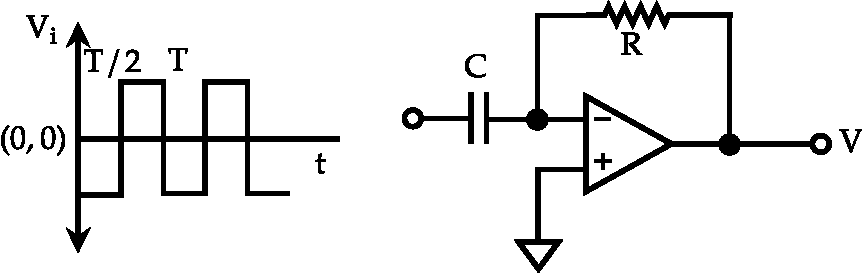
\includegraphics[height=3cm,width=8cm]{e73}
	\end{figure}
	Which of the waveforms $V_0$ best describes the output?
	{	\exyear{NET/JRF(JUNE-2018)}}
	\begin{tasks}(2)
		\task[\textbf{A.}] \begin{figure}[H]
			\centering
			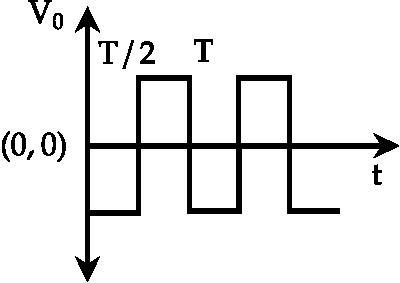
\includegraphics[height=3cm,width=5cm]{e73a}
		\end{figure}
		\task[\textbf{B.}] \begin{figure}[H]
			\centering
			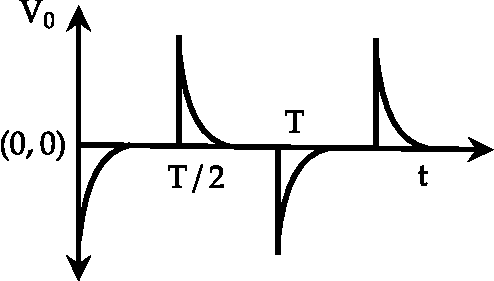
\includegraphics[height=3cm,width=5cm]{e73b}
		\end{figure}
		\task[\textbf{C.}] \begin{figure}[H]
			\centering
			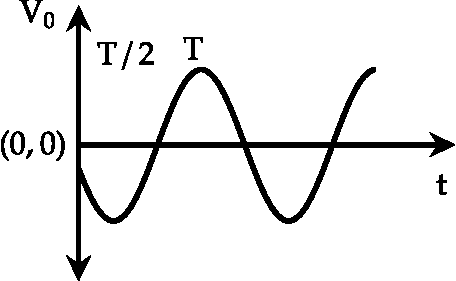
\includegraphics[height=3cm,width=5cm]{e73c}
		\end{figure}
		\task[\textbf{D.}] \begin{figure}[H]
			\centering
			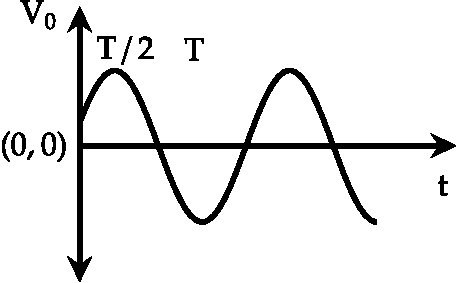
\includegraphics[height=3cm,width=5cm]{e73d}
		\end{figure}
	\end{tasks}
\begin{answer}$\left. \right. $\\
	It’s a differentiator circuit\\
	So the correct answer is \textbf{Option (B)}
\end{answer}
	\item The input $V_ i$ to the following circuit is a square wave as shown in the following figure.\\
	\begin{figure}[H]
		\centering
		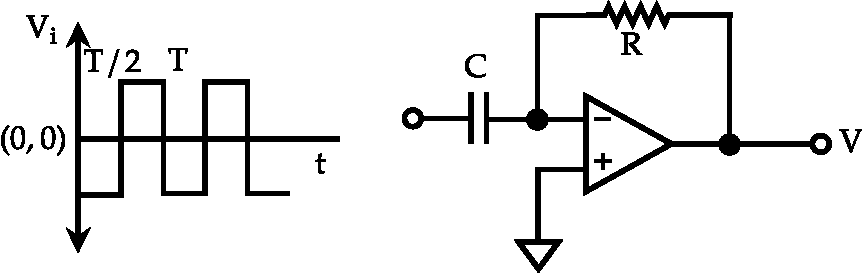
\includegraphics[height=2.5cm,width=8cm]{e73}
	\end{figure}
	which of the waveforms best describes the output?
	{	\exyear{NET/JRF(DEC-2018)}}
	\begin{tasks}(2)
		\task[\textbf{A.}] \begin{figure}[H]
			\centering
			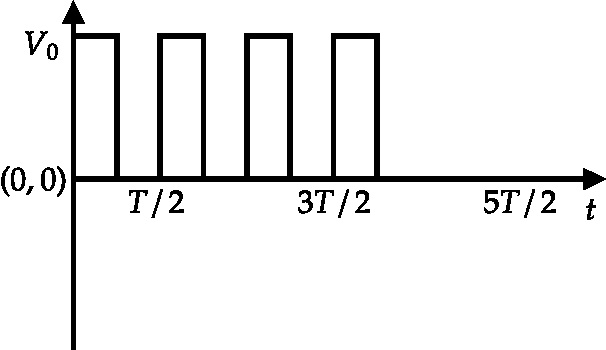
\includegraphics[height=3cm,width=5cm]{e74a}
		\end{figure}
		\task[\textbf{B.}] \begin{figure}[H]
			\centering
			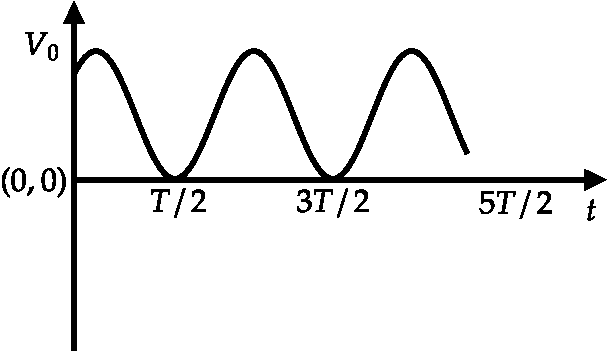
\includegraphics[height=3cm,width=5cm]{e74b}
		\end{figure}
		\task[\textbf{C.}] \begin{figure}[H]
			\centering
			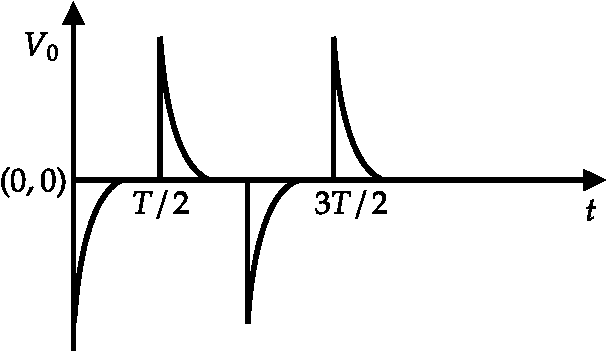
\includegraphics[height=3cm,width=5cm]{e74c}
		\end{figure}
		\task[\textbf{D.}]\begin{figure}[H]
			\centering
			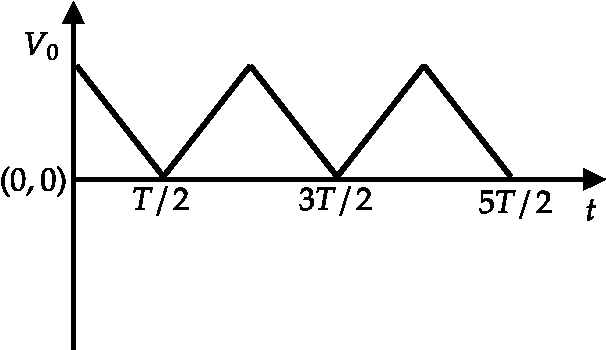
\includegraphics[height=3cm,width=5cm]{e74d}
		\end{figure}
	\end{tasks}
\begin{answer}
	Differentiator circuit.\\
	So the correct answer is \textbf{Option (C)}
\end{answer}
	\item A circuit constructed using op-amp, resistor $R_{1}=1 \mathrm{k} \Omega$ and capacitors $C_{1}=1 \mu \mathrm{F}$ and $C_{2}=0.1 \mu F$ is shown in the figure below.\\
	\begin{figure}[H]
		\centering
		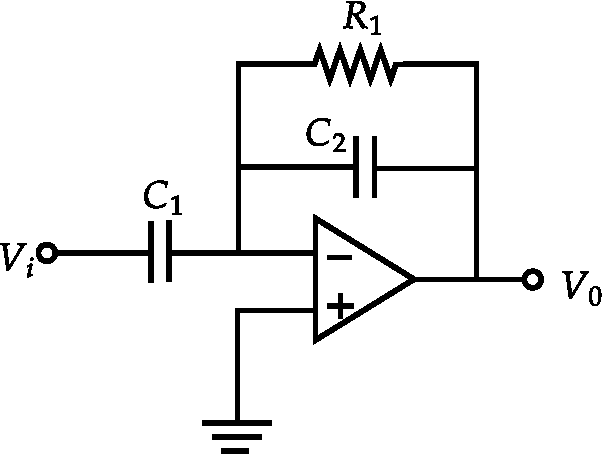
\includegraphics[height=4cm,width=5cm]{diagram-20211029(7)-crop}
	\end{figure}
	This circuit will act as a
	{	\exyear{NET/JRF(JUNE-2019)}}
	\begin{tasks}(2)
		\task[\textbf{A.}] High pass filter
		\task[\textbf{B.}] Low pass filter
		\task[\textbf{C.}] Band pass filter
		\task[\textbf{D.}] Band reject filter
	\end{tasks}
\begin{answer}
	\begin{align*}
	\frac{v_{0}}{v_{i}}&=-\frac{Z_{F}}{Z_{1}}=-\frac{\frac{R_{1} X_{C_{2}}}{R_{1}+X_{C_{2}}}}{X_{C_{1}}}=-\frac{R_{1}}{R_{1} / X_{C_{2}}+1} \times \frac{1}{1 / J \omega C_{1}}\\
	\Rightarrow \frac{v_{0}}{v_{i}}&=-\frac{R_{1} j \omega C_{1}}{R_{1} \times j \omega C_{2}+1}=\frac{R_{1} \omega C_{1}}{\sqrt{1+R_{1}^{2} \omega^{2} C_{2}^{2}}} \frac{e^{-j \theta_{1}}}{e^{j \theta_{2}}}\\
	\Rightarrow\left|\frac{v_{0}}{v_{i}}\right|&=\frac{R_{1} \omega C_{1}}{\sqrt{1+R_{1}^{2} \omega^{2} C_{2}^{2}}}=\frac{R_{1} C_{1}}{\sqrt{1 / \omega^{2}+R_{1}^{2} C_{2}^{2}}}\\
	\text{If }&\omega \rightarrow 0,\left|\frac{v_{0}}{v_{i}}\right| \rightarrow 0\text{ and If }\omega \rightarrow \infty\left|\frac{v_{0}}{v_{i}}\right| \rightarrow \frac{C_{1}}{C_{2}}
	\end{align*}
	So the correct answer is \textbf{Option (A)}
\end{answer}
	\item In the circuit diagram of a band pass filter shown below, $R=10 \mathrm{k} \Omega$.\\
	\begin{figure}[H]
		\centering
		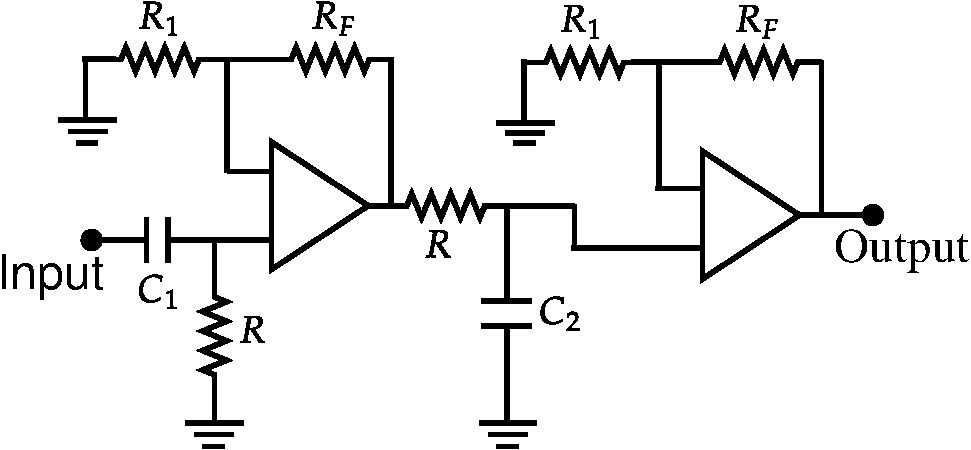
\includegraphics[height=3.5cm,width=8cm]{diagram-20211029(10)-crop}
	\end{figure}
	In order to get a lower cut-off frequency of $150 \mathrm{~Hz}$ and an upper cut-off frequency of $10 \mathrm{kHz}$, the appropriate values of $C_{1}$ and $C_{2}$ respectively are
	{	\exyear{NET/JRF(DEC-2019)}}
	\begin{tasks}(2)
		\task[\textbf{A.}]  $0.1 \mu F$ and $1.5 n F$
		\task[\textbf{B.}] $0.3 \mu \mathrm{F}$ and $5.0 \mathrm{nF}$
		\task[\textbf{C.}] $1.5 n F$ and $0.1 \mu F$
		\task[\textbf{D.}]  $5.0 \mathrm{nF}$ and $0.3 \mu \mathrm{F}$
	\end{tasks}
\begin{answer}
	\begin{align*}
	\text{Lower cut -off frequency of }H . P . F&=\frac{1}{2 \pi R C_{1}}=10 H z\\
	\Rightarrow C_{1}&=\frac{1}{2 \pi \times 10 \times 10^{3} \times 10} \approx 0.1 \mu \mathrm{F}\\
	\text{Higher cut-off frequency of }L . P . F&=\frac{1}{2 \pi R C_{2}}=10 \times 10^{3} \mathrm{~Hz}\\
	\Rightarrow C_{2}&=\frac{1}{2 \pi \times 10 \times 10^{3} \times 10^{4}} \approx 1.5 n F
	\end{align*}
	So the correct answer is \textbf{Option (A)}
\end{answer}
	\item The $I-V$ characteristics of the diode $D$ in the circuit below is given by
	$$
	I=I_{s}\left(e^{\frac{q V}{k_{\mathrm{B}} T}}-1\right)
	$$
	where $I_{s}$ is the reverse saturation current, $V$ is the voltage across the diode and $T$ is the absolute temperature.\\
	\begin{figure}[H]
		\centering
		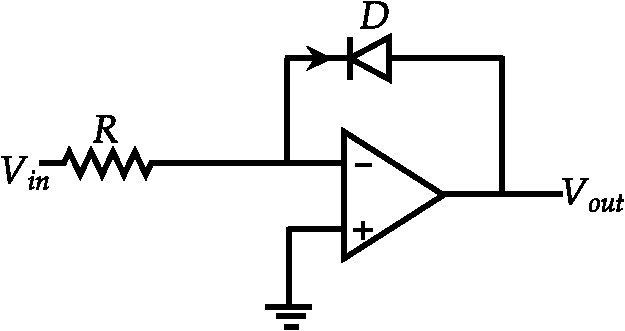
\includegraphics[height=3.5cm,width=6cm]{diagram-20211030(4)-crop}
		\caption{}
		\label{}
	\end{figure}
	If the input voltage is $V_{\text {in }}$, then the output voltage $V_{\text {out }}$ is
	{	\exyear{NET/JRF(JUNE-2020)}}
	\begin{tasks}(2)
		\task[\textbf{A.}] (a) $I_{s} R \ln \left(\frac{q V_{\text {in }}}{k_{B} T}+1\right)$
		\task[\textbf{B.}] $\frac{1}{q} k_{B} T \ln \left(\frac{q\left(V_{\text {in }}+I_{s} R\right)}{k_{B} T}\right)$
		\task[\textbf{C.}]  $\frac{1}{q} k_{B} T \ln \left(\frac{V_{\text {in }}}{I_{s} R}+1\right)$
		\task[\textbf{D.}]  $-\frac{1}{q} k_{B} T \ln \left(\frac{V_{\text {in }}}{I_{s} R}+1\right)$
	\end{tasks}
\begin{answer}
	\begin{align*}
	\because I&=I_{R} \quad \Rightarrow I_{S}\left(e^{e V_{D} / k_{B} T}-1\right)=\frac{0-\left(-V_{i n}\right)}{R}\\
	\\\Rightarrow e^{e V_{D} / k_{B} T}-1&=+\frac{V_{i n}}{I_{S} R} \Rightarrow e^{e V_{D} / k_{B} T}\\&=\frac{V_{i n}}{I_{S} R}+1 \Rightarrow V_{D}=\frac{k_{B} T}{e} \ln \left(\frac{V_{\text {in }}}{I_{S} R}+1\right)
	\end{align*}
	So the correct answer is \textbf{Option (C)}
\end{answer}
	\item In the circuit shown below, the gain of the op-amp in the middle of its bandwidth is $10^{5}$. A sinusoidal voltage with angular frequency $\omega=100 \mathrm{rad} / \mathrm{s}$ is applied to the input of the op-amp.\\
	\begin{figure}[H]
		\centering
		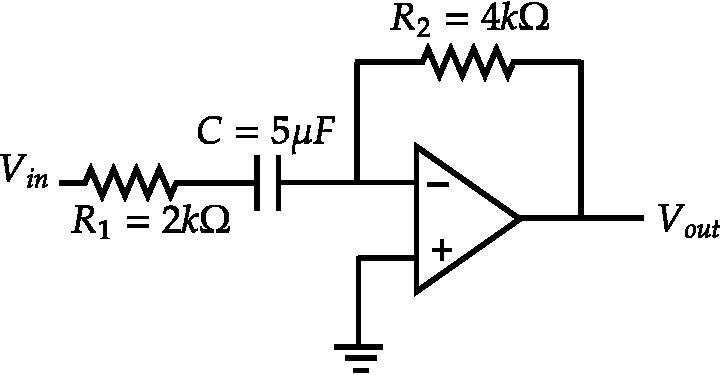
\includegraphics[height=4cm,width=7cm]{diagram-20211030(5)-crop}
		\caption{}
		\label{}
	\end{figure}
	The phase difference between the input and the output voltage is
	{	\exyear{NET/JRF(JUNE-2020)}}
	\begin{tasks}(4)
		\task[\textbf{A.}]  $5 \pi / 4$
		\task[\textbf{B.}] $3 \pi / 4$
		\task[\textbf{C.}] $\pi / 2$
		\task[\textbf{D.}] $\pi$
	\end{tasks}
\begin{answer}
	\begin{align*}
	\frac{v_{0}}{v_{m}}&=\frac{-R_{2}}{R_{1}+X_{C}} \Rightarrow \frac{v_{0}}{v_{m}}=\frac{-4 \times 10^{3}}{2 \times 10^{3}+\frac{1}{j \times 100 \times 5 \times 10^{-6}}}\\&=\frac{4}{2-2 j}=-\frac{4}{\sqrt{4+4} e^{-j \pi / 4}}=-\sqrt{2} e^{j \pi / 4}\\
	\Rightarrow \frac{v_{0}}{v_{m}}&=\sqrt{2} e^{j \pi} e^{j \pi / 4}=\sqrt{2} e^{j 5 \pi / 4}\\
	&\Rightarrow\text{ Input lags output by }\frac{5 \pi}{4}
	\end{align*}
	So the correct answer is \textbf{Option (A)}
\end{answer}
\end{enumerate}
\newpage
\begin{abox}
	Practice Set- 2
\end{abox}
\begin{enumerate}
	\item In one of the following circuits, negative feedback does not operate for a negative input. Which one is it? The opamps are running from $\pm 15 \mathrm{~V}$ supplies.
	{\exyear{GATE 2010}}
\begin{tasks}(2)
\task[\textbf{A.}] \begin{figure}[H]
	\centering
	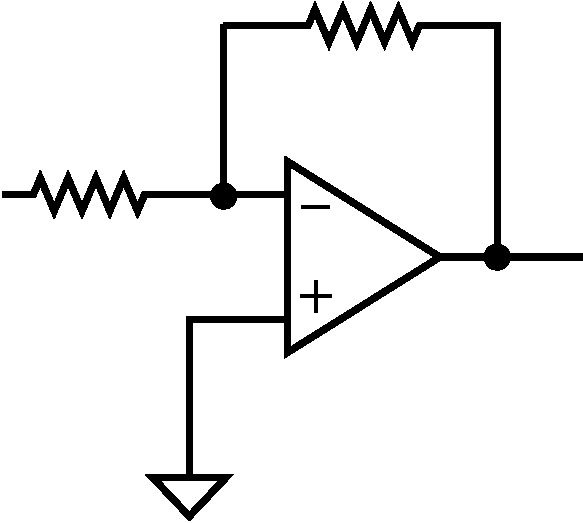
\includegraphics[height=3.5cm,width=4cm]{diagram-20210912(9)-crop}
\end{figure}
\task[\textbf{B.}] \begin{figure}[H]
	\centering
	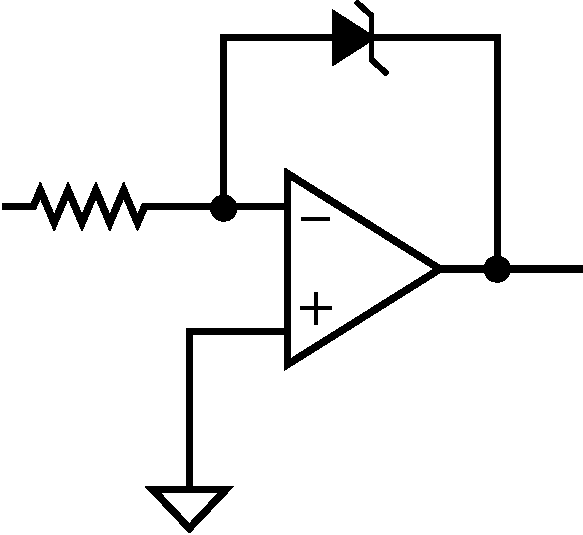
\includegraphics[height=3.5cm,width=4cm]{diagram-20210912(10)-crop}
\end{figure}
\task[\textbf{C.}] \begin{figure}[H]
	\centering
	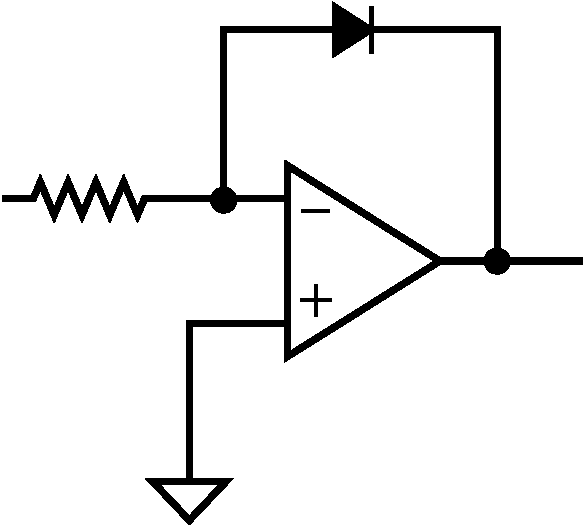
\includegraphics[height=3.5cm,width=4cm]{diagram-20210912(11)-crop}
\end{figure}
\task[\textbf{D.}] \begin{figure}[H]
	\centering
	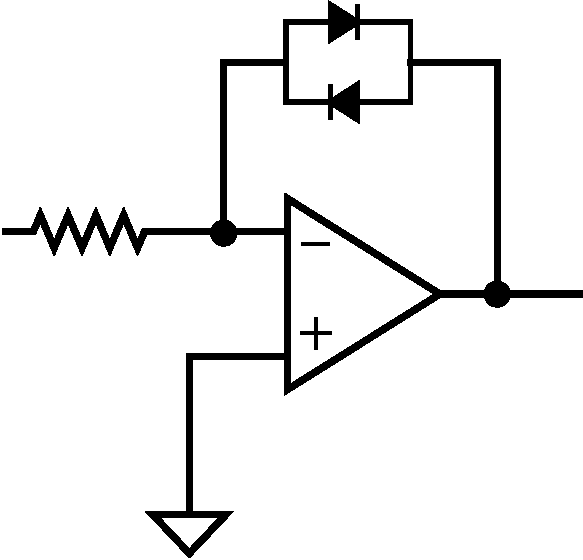
\includegraphics[height=3.5cm,width=4cm]{diagram-20210912(12)-crop}
\end{figure}
\end{tasks}
\begin{answer}
So the correct answer is \textbf{Option (C)}
\end{answer}
	\item Consider the following circuit.\\
	\begin{figure}[H]
		\centering
		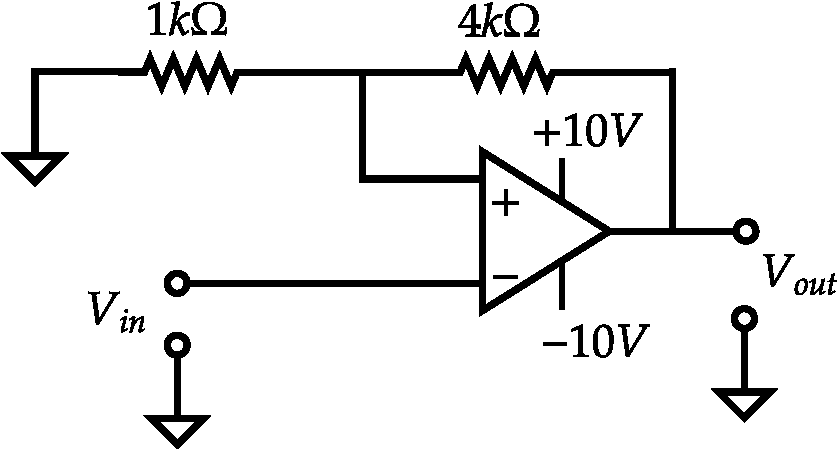
\includegraphics[height=4cm,width=7.5cm]{diagram-20210913(6)-crop}
	\end{figure}
	Which of the following correctly represents the output $V_{\text {out }}$ corresponding to the input $V_{i n} ?$
	{\exyear{GATE 2011}}
\begin{tasks}(2)
\task[\textbf{A.}] \begin{figure}[H]
	\centering
	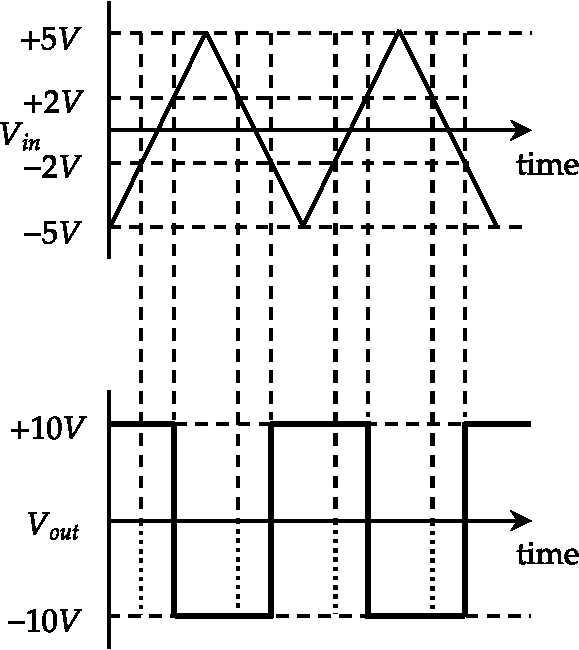
\includegraphics[height=6.5cm,width=6cm]{diagram-20210913(2)-crop}
\end{figure}
\task[\textbf{B.}] \begin{figure}[H]
	\centering
	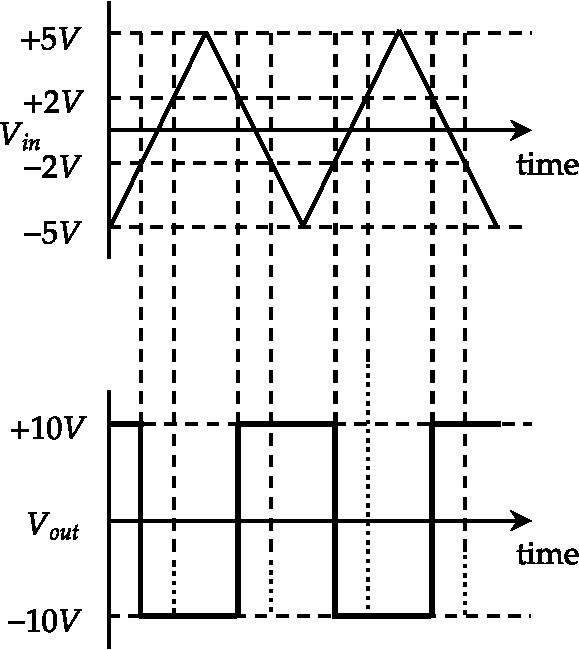
\includegraphics[height=6.5cm,width=6cm]{diagram-20210913(3)-crop}
\end{figure}
\task[\textbf{C.}]\begin{figure}[H]
	\centering
	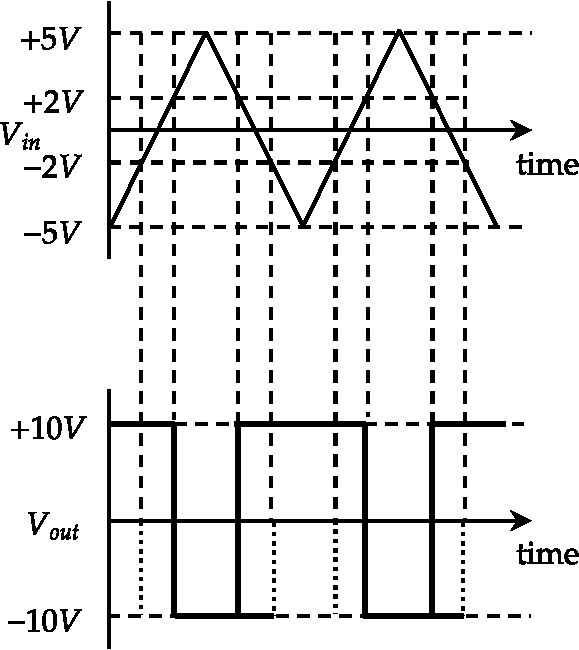
\includegraphics[height=6.5cm,width=6cm]{diagram-20210913(4)-crop}
\end{figure}
\task[\textbf{D.}] \begin{figure}[H]
	\centering
	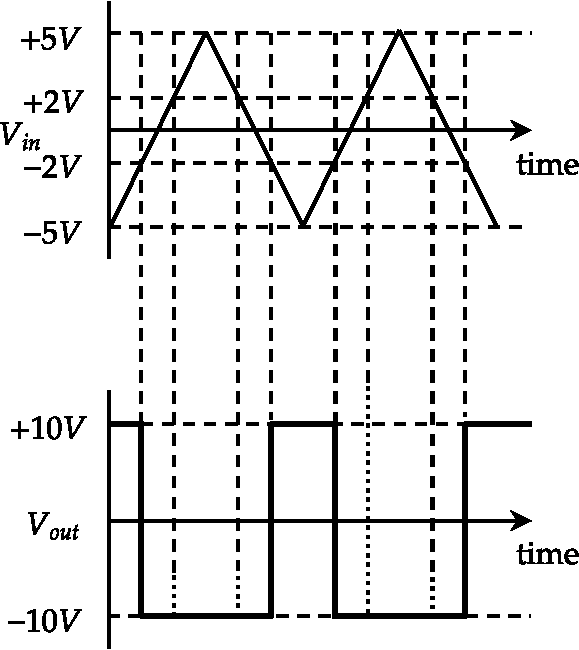
\includegraphics[height=6.5cm,width=6cm]{diagram-20210913(5)-crop}
\end{figure}
\end{tasks}
\begin{answer}
\begin{align*}
V_{u t}&=\left(\frac{1}{1+4}\right) \times 10=+2 V, \\ V_{l t}&=\left(\frac{1}{1+4}\right) \times-10=-2 V
\end{align*}
So the correct answer is \textbf{Option (A)}
\end{answer}
	\item If the peak output voltage of a full wave rectifier is $10 \mathrm{~V}$, its d.c. voltage is
{	\exyear{GATE 2012}}
\begin{tasks}(4)
\task[\textbf{A.}] $10.0 \mathrm{~V}$
\task[\textbf{B.}] $7.07 \mathrm{~V}$
\task[\textbf{C.}] $6.36 \mathrm{~V}$
\task[\textbf{D.}] $3.18 \mathrm{~V}$
\end{tasks}
\begin{answer}
\begin{align*}
V_{d c}&=\frac{2 V_{m}}{\pi}=\frac{2 \times 10}{22 / 7}\\&=\frac{14 \times 10}{22}=\frac{70}{11}=6.36 \mathrm{~V}
\end{align*}
So the correct answer is \textbf{Option (C)}
\end{answer}
	\item In the following circuit, for the output voltage to be $V_{0}=\left(-V_{1}+V_{2} / 2\right)$ the ratio $R_{1} / R_{2}$ is
{	\exyear{GATE 2012}}
\begin{figure}[H]
\centering
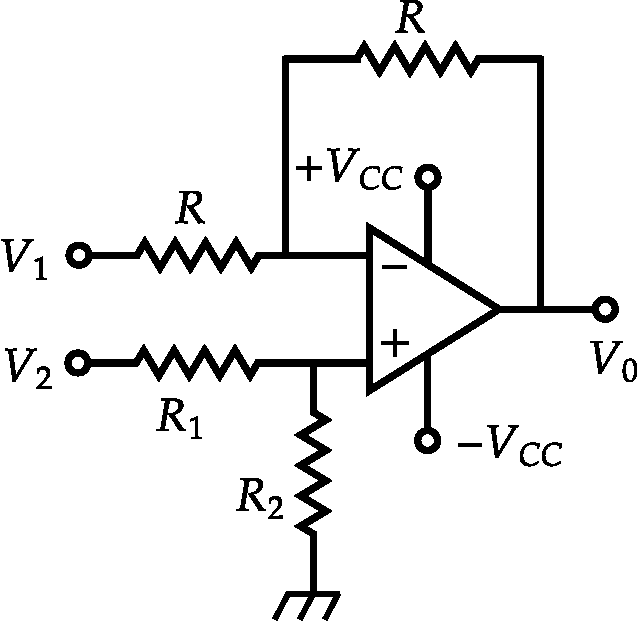
\includegraphics[height=6.5cm,width=6.5cm]{diagram-20210913(12)-crop}
\end{figure}
\begin{tasks}(4)
\task[\textbf{A.}] $1 / 2$
\task[\textbf{B.}] 1
\task[\textbf{C.}] 2
\task[\textbf{D.}] 3
\end{tasks}
\begin{answer}
\begin{align*}
\text{	When }V_{2}&=0, \quad v_{01}=-V_{1}\\
\text{when }V_{1}&=0, \quad v_{02}=\left(1+\frac{R}{R}\right)\left(\frac{R_{2}}{R_{1}+R_{2}}\right) V_{2}\\
\text{Since }V_{0}&=-V_{1}+\frac{V_{2}}{2} \Rightarrow 2 \cdot \frac{R_{2}}{R_{1}+R_{2}}=\frac{1}{2} \Rightarrow \frac{R_{1}}{R_{2}}=3
\end{align*}
So the correct answer is \textbf{Option (D)}
\end{answer}
	\item Consider the following OP-AMP circuit.
	Which one of the following correctly represents the output $\mathrm{V}_{\text {out }}$ corresponding to the input $\mathrm{V}_{\text {in }}$ ?
{	\exyear{GATE 2012}}
\begin{figure}[H]
\centering
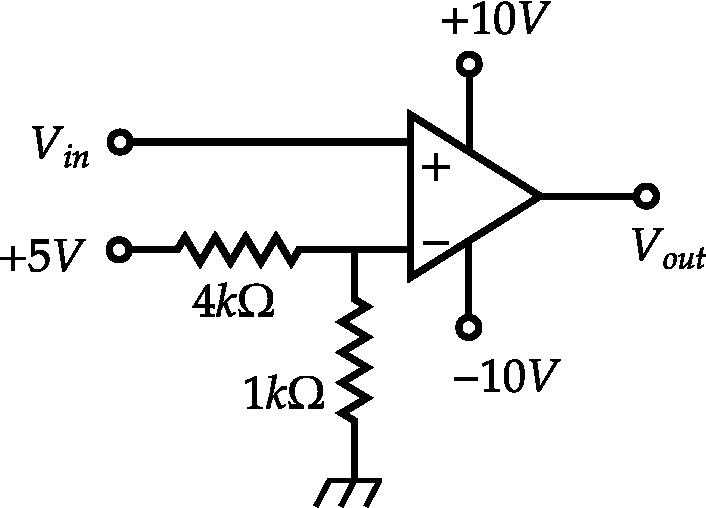
\includegraphics[height=5.5cm,width=7cm]{diagram-20210913(13)-crop}
\end{figure}
\begin{tasks}(2)
\task[\textbf{A.}] \begin{figure}[H]
	\centering
	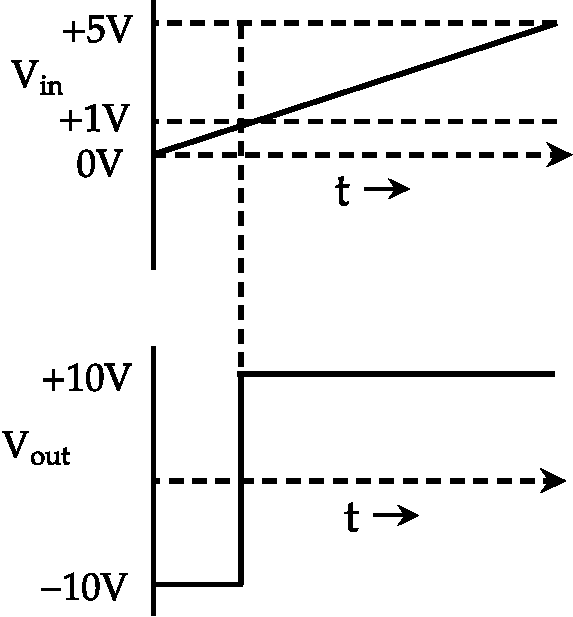
\includegraphics[height=6cm,width=5cm]{diagram-20210913(15)-crop}
\end{figure}
\task[\textbf{B.}] \begin{figure}[H]
	\centering
	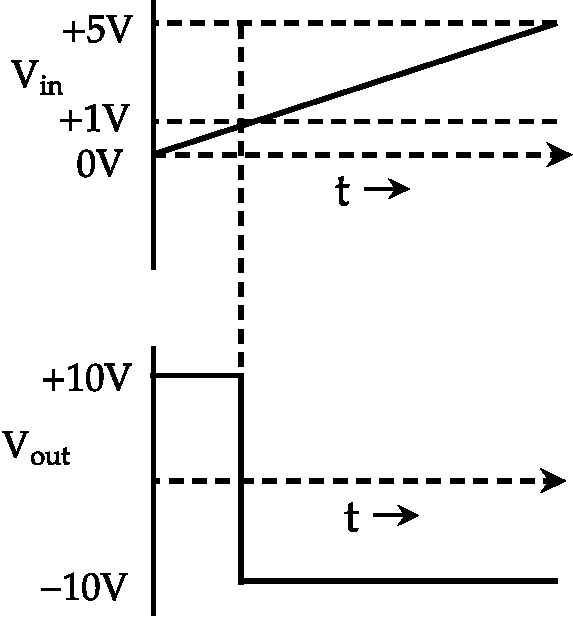
\includegraphics[height=6cm,width=5cm]{diagram-20210913(16)-crop}
\end{figure}
\task[\textbf{C.}] \begin{figure}[H]
	\centering
	\includegraphics[height=6cm,width=5cm]{diagram-20210913(17)-crop}
\end{figure}
\task[\textbf{D.}] \begin{figure}[H]
	\centering
	\includegraphics[height=6cm,width=5cm]{diagram-20210913(18)-crop}
\end{figure}
\end{tasks}
\begin{answer}
\begin{align*}
\text{Voltage at inverting input }V_{2}&=\left(\frac{1}{1+4}\right) \times 5=+1 V\\
\text{	When }v_{i n}>+1 V, \quad v_{0}&=+V_{C C}\text{ and when }v_{i n}<+1 V, \quad v_{0}=-V_{C C}
\end{align*}
So the correct answer is \textbf{Option (A)}
\end{answer}
	\item For this circuit the frequency above which the gain will decrease by $20 d B$ per decade is
{	\exyear{GATE 2013}}
\begin{figure}[H]
\centering
\includegraphics[height=5cm,width=9cm]{diagram-20210913(28)-crop}
\end{figure}
\begin{tasks}(4)
\task[\textbf{A.}] $15.9 \mathrm{kHz}$
\task[\textbf{B.}] $1.2 \mathrm{kHz}$
\task[\textbf{C.}]  $5.6 \mathrm{kHz}$
\task[\textbf{D.}] $22.5 \mathrm{kHz}$
\end{tasks}
\begin{answer}
\begin{align*}
f_{H}&=\frac{1}{2 \pi R C}=16 \mathrm{kHz}
\end{align*}
So the correct answer is \textbf{Option (A)}
\end{answer}
\item At $1.2 \mathrm{kHz}$ the closed loop gain is
{\exyear{GATE 2013}}
\begin{tasks}(4)
\task[\textbf{A.}] 1
\task[\textbf{B.}] $1.5$
\task[\textbf{C.}]  3
\task[\textbf{D.}]  $0.5$
\end{tasks}
\begin{answer}
\begin{align*}
\left|\frac{v_{0}}{v_{i n}}\right|&=\frac{\left(1+R_{F} / R_{1}\right)}{\sqrt{1+\left(f / f_{H}\right)^{2}}}=1.5
\end{align*}
So the correct answer is \textbf{Option (B)}
\end{answer}
	\item The input given to an ideal OP-AMP integrator circuit is\\
	\begin{figure}[H]
		\centering
		\includegraphics[height=3cm,width=6cm]{diagram-20210913(29)-crop}
	\end{figure}
	The correct output of the integrator circuit is
{	\exyear{GATE 2014}}
\begin{tasks}(2)
\task[\textbf{A.}] \begin{figure}[H]
	\centering
	\includegraphics[height=3cm,width=6cm]{diagram-20210913(30)-crop}
\end{figure}
\task[\textbf{B.}] \begin{figure}[H]
	\centering
	\includegraphics[height=3cm,width=6cm]{diagram-20210913(31)-crop}
\end{figure}
\task[\textbf{C.}] \begin{figure}[H]
	\centering
	\includegraphics[height=3cm,width=6cm]{diagram-20210913(32)-crop}
\end{figure}
\task[\textbf{D.}] \begin{figure}[H]
	\centering
	\includegraphics[height=3cm,width=6cm]{diagram-20210913(33)-crop}
\end{figure}
\end{tasks}
\begin{answer}
So the correct answer is \textbf{Option (A)}
\end{answer}
	\item A low pass filter is formed by a resistance $R$ and a capacitance $C .$ At the cut-off angular frequency $\omega_{C}=\frac{1}{R C}$ the voltage gain and the phase of the output voltage relative to the input voltage respectively are
{	\exyear{GATE 2014}}
\begin{tasks}(4)
\task[\textbf{A.}] $0.71$ and $45^{\circ}$
\task[\textbf{B.}]  $0.71$ and $-45^{\circ}$
\task[\textbf{C.}] $0.5$ and $-90^{\circ}$
\task[\textbf{D.}] $0.5$ and $90^{\circ}$
\end{tasks}
\begin{answer}
\begin{align*}
\frac{v_{0}}{v_{i n}}&=\frac{X_{C}}{R+X_{C}}=\frac{1}{\frac{R}{X_{C}}+1}\\&=\frac{1}{1+j \omega C R}\\
At \omega&=\omega_{C}=\frac{1}{R C} \Rightarrow \frac{v_{0}}{v_{i n}}=\frac{1}{1+j}\\&=\frac{1}{\sqrt{2} e^{j 45^{0}}}=\frac{1}{\sqrt{2}} e^{-j 45^{0}}
\end{align*}
So the correct answer is \textbf{Option (B)}
\end{answer}
	\item Consider the circuit shown in the figure, where $R C=1$. For an input signal $V_{i}$ shown below, choose the correct $V_{0}$ from the options:
{	\exyear{GATE 2015}}
\begin{figure}[H]
\centering
\includegraphics[height=4.5cm,width=12cm]{diagram-20210913(42)-crop}
\end{figure}
\begin{tasks}(2)
\task[\textbf{A.}] \begin{figure}[H]
	\centering
	\includegraphics[height=4.5cm,width=6.5cm]{diagram-20210913(37)-crop}
\end{figure}
\task[\textbf{B.}] \begin{figure}[H]
	\centering
	\includegraphics[height=4.5cm,width=6.5cm]{diagram-20210913(38)-crop}
\end{figure}
\task[\textbf{C.}] \begin{figure}[H]
	\centering
	\includegraphics[height=4.5cm,width=6.5cm]{diagram-20210913(39)-crop}
\end{figure}
\task[\textbf{D.}]\begin{figure}[H]
	\centering
	\includegraphics[height=4.5cm,width=6.5cm]{diagram-20210913(40)-crop}
\end{figure}
\end{tasks}
\begin{answer}
\begin{align*}
C \frac{d v_{i}}{d t}&=\frac{0-v_{0}}{R} \Rightarrow v_{0}=-R C \frac{d v_{i n}}{d t}\\&=-\frac{d v_{i n}}{d t} \Rightarrow v_{i n}=-v_{0} t\\
v_{i n}&=+t \Rightarrow v_{0}=-1 V \quad\text{ and }v_{i n}\\&=-t \Rightarrow v_{0}=+1 V
\end{align*}
So the correct answer is \textbf{Option (B)}
\end{answer}
	\item In the given circuit, if the open loop gain $A=10^{5}$ the feedback configurations and the closed loop gain $A_{f}$ are
{	\exyear{GATE 2015}}
\begin{figure}[H]
\centering
\includegraphics[height=4cm,width=6cm]{diagram-20210914(2)-crop}
\end{figure}
\begin{tasks}(2)
\task[\textbf{A.}] series-shunt, $A_{f}=9$
\task[\textbf{B.}] series-series, $A_{f}=10$
\task[\textbf{C.}] series-shunt, $A_{f}=10$
\task[\textbf{D.}] shunt-shunt, $A_{f}=10$
\end{tasks}
\begin{answer}
\begin{align*}
A_{F}&=\left(1+\frac{R_{F}}{R_{1}}\right)=(1+9)=10
\end{align*}
So the correct answer is \textbf{Option (C)}
\end{answer}
	\item Consider an ideal operational amplifier as shown in the figure below with $R_{1}=5 k \Omega, R_{2}=1 k \Omega, R_{L}=100 k \Omega .$ For an applied input voltage $V=10 \mathrm{mV}$, the current passing through $R_{2}$ is............... $\mu A$. (up to two decimal places)
	{\exyear{GATE 2017}}
\begin{figure}[H]
\centering
\includegraphics[height=4cm,width=6.5cm]{diagram-20210914(12)-crop}
\end{figure}
\begin{answer}
\begin{align*}
I_{2}&=\frac{V}{R_{2}}=\frac{10}{1}=10 \mu A
\end{align*}
\end{answer}
	\item For an operational amplifier (ideal) circuit shown below,\\
	\begin{figure}[H]
		\centering
		\includegraphics[height=4cm,width=7cm]{diagram-20210914(30)-crop}
		\caption{}
		\label{}
	\end{figure}
	If $V_{1}=1 V$ and $V_{2}=2 V$, the value of $V_{0}$ is ---------$V$ (up to one decimal place).
{	\exyear{GATE 2018}}
\begin{answer}
\begin{align*}
V_{0}&=V_{01}+V_{02}=-\frac{4}{2} \times 1 V-\frac{4}{5} \times 2 V\\
V_{0}&=-2-1.6=-3.6 \mathrm{~V}
\end{align*}
\end{answer}
	\item For the following circuit, what is the magnitude of $V_{\text {out }}$ if $V_{\text {in }}=1.5 V$ ?
{	\exyear{IIT JAM 2018}}
\begin{figure}[H]
\centering
\includegraphics[height=5cm,width=7cm]{diagram-20210914(21)-crop}
\end{figure}
\begin{tasks}(4)
\task[\textbf{A.}] $0.015 \mathrm{~V}$
\task[\textbf{B.}] $0.15 \mathrm{~V}$
\task[\textbf{C.}] $15 \mathrm{~V}$
\task[\textbf{D.}] $150 \mathrm{~V}$
\end{tasks}
\begin{answer}
\begin{align*}
V_{o u t}&=-\frac{100 R}{R} \times 1.5=-150 \mathrm{~V} \Rightarrow\left|V_{0}\right|=15 \mathrm{~V}
\end{align*}
So the correct answer is \textbf{Option (C)}
\end{answer}
	\item What is the voltage at the output of the following operational amplifier circuit. [See in the figure]?
{	\exyear{JEST 2015}}
\begin{figure}[H]
\centering
\includegraphics[height=5.5cm,width=7cm]{diagram-20210816(10)-crop}
\end{figure}
\begin{tasks}(4)
\task[\textbf{A.}] $1 \mathrm{~V}$
\task[\textbf{B.}] $1 \mathrm{mV}$
\task[\textbf{C.}] $1 \mu V$
\task[\textbf{D.}] $1 n V$
\end{tasks}
\begin{answer}
\begin{align*}
\text{Output of first Op-Amp }v_{01}&=-\left(10 \times 10^{3}\right)\left(1 \times 10^{-9}\right)\\&=-10^{-5} volt\\
\text{	Output of first Op-Amp }v_{\text {out }}&=\left(1+\frac{99}{1}\right) \times 10^{-5}\\&=10^{-3} volts =1 \mathrm{mV}
\end{align*}
So the correct answer is \textbf{Option (B)}
\end{answer}
	\item Consider a 741 operational amplifier circuit as shown below, where $V_{C C}=V_{E E}=+15 V$ and $R=2.2 \mathrm{k} \Omega$. If $v_{I}=2 m V$, what is the value of $v_{0}$ with respect to the ground?
{	\exyear{JEST 2017}}
\begin{figure}[H]
\centering
\includegraphics[height=5.5cm,width=7cm]{diagram-20210816(29)-crop}
\end{figure}
\begin{tasks}(4)
\task[\textbf{A.}] $-1 \mathrm{mV}$
\task[\textbf{B.}] $-2 m V$
\task[\textbf{C.}] $-3 m V$
\task[\textbf{D.}] $-4 m V$
\end{tasks}
\begin{answer}
Apply KCL;
\begin{figure}[H]
	\centering
	\includegraphics[height=5.5cm,width=8cm]{diagram-20210816(30)-crop}
\end{figure}
\begin{align*}
I_{1}&=I_{2} \Rightarrow \frac{v_{i}-0}{R}=\frac{0-v_{0}}{3 R / 2}\\
\Rightarrow v_{0}&=-\frac{3}{2} v_{i}=-\frac{3}{2} \times 2\\&=-3 m V
\end{align*}
So the correct answer is \textbf{Option (C)}
\end{answer}
	\item Analyse the ideal op-amp circuit in the figure. Which one of the following statements is true about the output voltage $V_{\text {out }}$, when terminal ' $C$ ' is connected to point ' $A$ ' and then to point ' $B$ '?
	{\exyear{JEST 2019}}
\begin{figure}[H]
\centering
\includegraphics[height=4.5cm,width=6cm]{diagram-20210817(1)-crop}
\end{figure}
\begin{tasks}(1)
\task[\textbf{A.}] $V_{\text {out }}=V_{\text {in }}$ and $V_{\text {out }}=-V_{\text {in }}$ when ' $C$ ' is connected to ' $A$ ' and ' $B$ ', respectively
\task[\textbf{B.}] $V_{\text {out }}=-V_{\text {in }}$ and $V_{\text {out }}=V_{\text {in }}$ when ' $C$ ' is connected to ' $A$ ' and ' $B$ ', respectively
\task[\textbf{C.}] $V_{\text {out }}=-V_{\text {in }}$ when ' $C$ ' is connected to either ' $A$ ' or ' $B$ '
\task[\textbf{D.}]  $V_{\text {out }}=V_{\text {in }}$ when ' $C$ ' is connected to either ' $A$ ' or ' $B$ '
\end{tasks}
\begin{answer}
\begin{align*}
\intertext{	When terminal ' $C$ ' is connected to point ' $A$ '}
V_{\text {out }}&=\left(1+\frac{1}{1}\right) V_{\text {in }}-\frac{1}{1} V_{\text {in }}=V_{\text {in }}
\intertext{When terminal ' $C$ ' is connected to point ' $B$ '}
V_{\text {out }}&=-\frac{1}{1} V_{\text {in }}=-V_{\text {in }}
\end{align*}
So the correct answer is \textbf{Option (A)}
\end{answer}
	
	
	
	
	
	
	
	
	
	
	
	
	
	
	
	
	
	
	
	
	
	
\end{enumerate}